\documentclass{beamer}
\usetheme{Warsaw}
\setbeamertemplate{headline}{}

\usepackage{ae,lmodern}
\usepackage[english]{babel}
\usepackage[utf8]{inputenc}
\usepackage[T1]{fontenc}

\usepackage{caption}
\captionsetup[figure]{labelformat=empty}

\PassOptionsToPackage{usenames,dvipsnames}{xcolor}
\usepackage{xcolor,colortbl}
\definecolor{DarkGrey}{HTML}{222222}
\definecolor{DarkBlue}{HTML}{004BA9}
\definecolor{DarkRed}{HTML}{CC1111}
\definecolor{DarkGreen}{HTML}{117711}
\definecolor{DarkOrange}{HTML}{CC7000}
\definecolor{LightGrey}{HTML}{DDDDDD}
\definecolor{LightBlue}{HTML}{F0F8FF}
\definecolor{codegreen}{rgb}{0,0.6,0}
\definecolor{codepurple}{rgb}{0.58,0,0.82}

\usepackage[cache=false]{minted}
\setminted[bash]{
   bgcolor=LightBlue,
   breaklines, breakanywhere,
   frame=single,
   autogobble
}
\usemintedstyle[python]{native}
\setminted[python]{
   bgcolor=black,
   breaklines, breakanywhere,
   autogobble
}

\usepackage{listings}
\usepackage{lstautogobble}
\lstdefinestyle{bash}{
    backgroundcolor=\color{DarkGrey},   
    commentstyle=\color{codegreen},
    keywordstyle=\color{magenta},
    numberstyle=\tiny\color{DarkGrey},
    stringstyle=\color{codepurple},
    basicstyle=\ttfamily\tiny\color{LightGrey},
    escapeinside={\%*}{*)},
    breakatwhitespace=false,         
    breaklines=true,                 
    captionpos=b,                    
    keepspaces=true,                 
    numbers=left,                    
    numbersep=5pt,                  
    showspaces=false,                
    showstringspaces=false,
    showtabs=false,
    showlines=false,
    tabsize=2
}

\usepackage{tikz}
\usetikzlibrary{calc,decorations.pathreplacing,arrows,arrows.meta,shapes,patterns, positioning}
\newcommand\BigLength{14.6em}
\newcommand\Height{2em}
\newcommand\Sep{0.6em}
\newcommand\Center{\BigLength*1/2}
\newcommand\BigBox{\BigLength+\Sep}
\newcommand\HalfBox{\BigLength*1/2-\Sep*1/4}
\newcommand\HalfLength{\BigLength*1/2-\Sep*5/4}
\newcommand\CenterL{\BigLength*1/4-\Sep*1/8}
\newcommand\CenterR{\BigLength*3/4+\Sep*1/8}
\tikzstyle{layer}=[rectangle,thick,text centered,
                     minimum height=\Height,minimum width=\BigLength]
\tikzstyle{short}=[rectangle,thick,text centered,
                     minimum height=\Height,minimum width=\HalfLength]
\tikzstyle{dibox}=[rectangle,thick,semitransparent,
                     minimum height=(\Height+\Sep)*2,minimum width=\BigBox]
\tikzstyle{vmbox}=[rectangle,thick,semitransparent,
                     minimum height=(\Height+\Sep)*3,minimum width=\HalfBox]
\tikzstyle{ctbox}=[rectangle,thick,semitransparent,
                     minimum height=(\Height+\Sep)*2,minimum width=\HalfBox]
\tikzstyle{vebox}=[rectangle,thick,semitransparent,
                     minimum height=(\Height+\Sep)*1,minimum width=\HalfBox]

\usepackage{hyperref}
\usepackage{grffile}


\AtBeginSection[]
{
   \begin{frame}
      \tableofcontents[currentsection]
   \end{frame}
}

\AtBeginSubsection[]
{
   \begin{frame}
      \tableofcontents[currentsection, currentsubsection, sectionstyle=shaded]
   \end{frame}
}

%----------------------------------------------------------------------------------------
\title{Introduction to Data Science}
\subtitle{with Python}
%----------------------------------------------------------------------------------------
\author{Alexis Bogroff}
\date{\today}



\begin{document}

\begin{frame}
   \titlepage
\end{frame}

\begin{frame}\frametitle{Presenter}
   \begin{minipage}{0.3\linewidth}
      \centering
      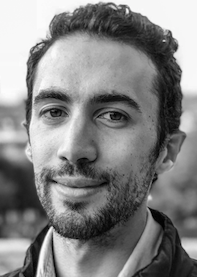
\includegraphics[width=0.6\textwidth]{../images/AlexisBogroff.png} \\
   \end{minipage}
   \begin{minipage}{0.6\linewidth}
      \noindent Alexis Bogroff \\
      Lecturer and Mentor in Data Science \\
      at Paris 1 Panthéon-Sorbonne, ESILV, Openclassrooms, EM-Lyon
   \end{minipage}
   \\[2ex]
   \visible<2->{\begin{itemize}
      \item 4 years Teaching Assistant and lecturer in VBA, Python for finance, SQL, Data Analysis and Data Science
      \item 9 months Researcher Assistant at Paris 1 Panthéon-Sorbonne within H2020 European Project
      \item 1 year Data Scientist at Pléiade Asset Management
   \end{itemize}}
   \hfill
\end{frame}

% \begin{frame}\frametitle{Overview}
%    \Large
%    \centering
%    Financial Engineering with Python Linux and Git \\[2ex]
%    \begin{minipage}{0.32\linewidth}
%       \includegraphics[width=0.8\textwidth]{../images/linux-1-logo-svg-vector.pdf}
%    \end{minipage}
%    \begin{minipage}{0.32\linewidth}
%       \includegraphics[width=0.8\textwidth]{../images/Git-logo.pdf}
%    \end{minipage}
%    \begin{minipage}{0.32\linewidth}
%       \includegraphics[width=0.9\textwidth]{../images/Python_logo_and_wordmark.pdf}
%    \end{minipage}
%    \pause
%    \\[3ex]
%    Free and everywhere stack \\
%    To find a job and be operational
% \end{frame}

% \begin{frame}\frametitle{Lecture Organisation}
%    \begin{itemize}[<+->]
%       \item Prerequisite:
%       \begin{enumerate}
%          \item Have a Linux environment working on your personal computer
%          \item[] (it can be WSL2 on Windows, Amazon EC2 for a distant solution)
%          \item Install Git
%          \item Install Python
%       \end{enumerate}
%       \vspace{2em}
%       \item Exam:
%       \begin{itemize}
%          \item Last QCM 1/2
%          \item Project 1/2
%       \end{itemize}
%    \end{itemize}
% \end{frame}


\begin{frame}
   \tableofcontents
\end{frame}

% =============================================================================
% =============================================================================
\section{Conclusion}
% 45min course
% =============================================================================
% =============================================================================


%------------------------------------------------------------------------------
\subsection{Recap: What to remember from this course}
%------------------------------------------------------------------------------



\begin{frame}\frametitle{Remember from this course}
   \begin{minipage}{0.48\linewidth}
      \begin{itemize}
         \item Overview
         \item Python
         \item Pandas
         \item Data Analysis
         \item Data Management with Pandas
         \item Data Visualization
         \item Predictions
      \end{itemize}
   \end{minipage}
   \begin{minipage}{0.48\linewidth}
      \begin{figure}[H]
         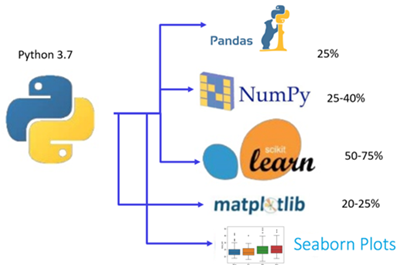
\includegraphics[scale=.45]{../images/illustrations/packages.png}
      \end{figure}
   \end{minipage}
\end{frame}

\begin{frame}\frametitle{Overview}
   \begin{minipage}{0.6\linewidth}
      \begin{itemize}
         \item Artificial Intelligence, Machine Learning, Deep Learning
         \item Computer Vision, Recommander systems, NLP
         \item Programming
         \item Data Analysis
         \item Issues, risks, ethics, RGPD
         \item Ressources
      \end{itemize}
   \end{minipage}
   \begin{minipage}{0.38\linewidth}
      \begin{figure}[H]
         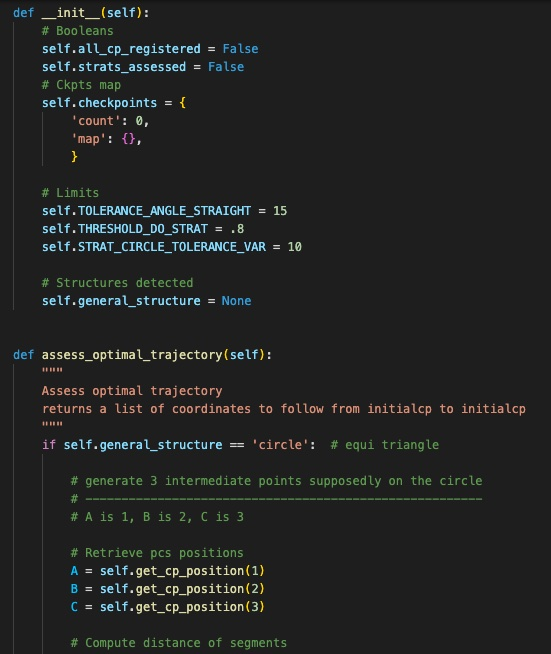
\includegraphics[scale=.17]{../images/illustrations/code.jpg}
      \end{figure}
   \end{minipage}

   \vspace{.5cm}
   \begin{minipage}{0.48\linewidth}
      \begin{figure}[H]
         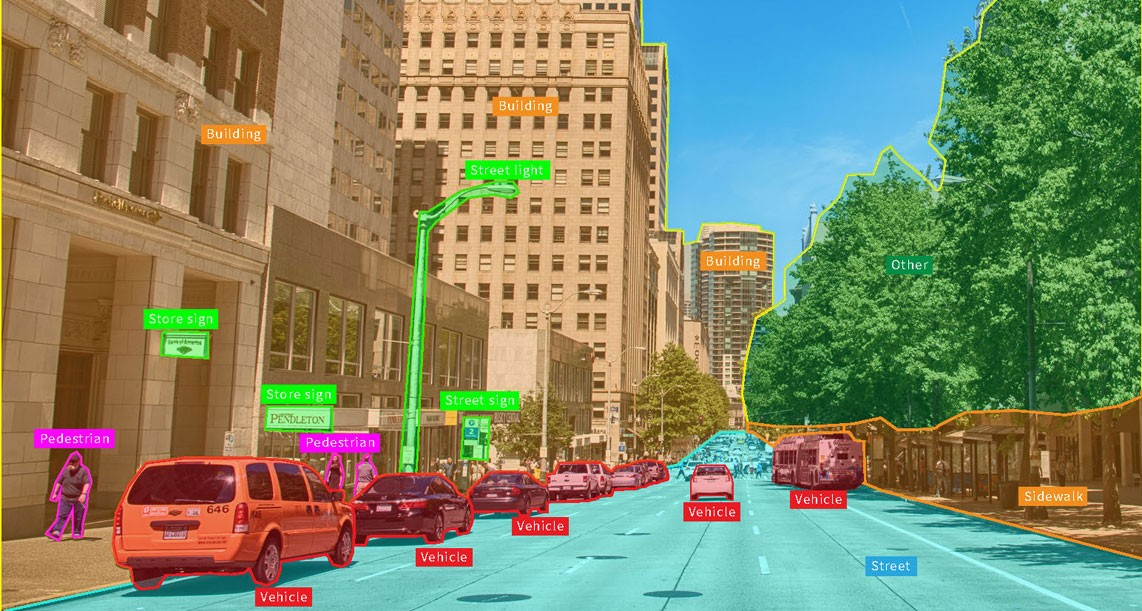
\includegraphics[scale=.1]{../images/illustrations/objects-detection.jpeg}
      \end{figure}
   \end{minipage}
   \begin{minipage}{0.48\linewidth}
      \begin{figure}[H]
         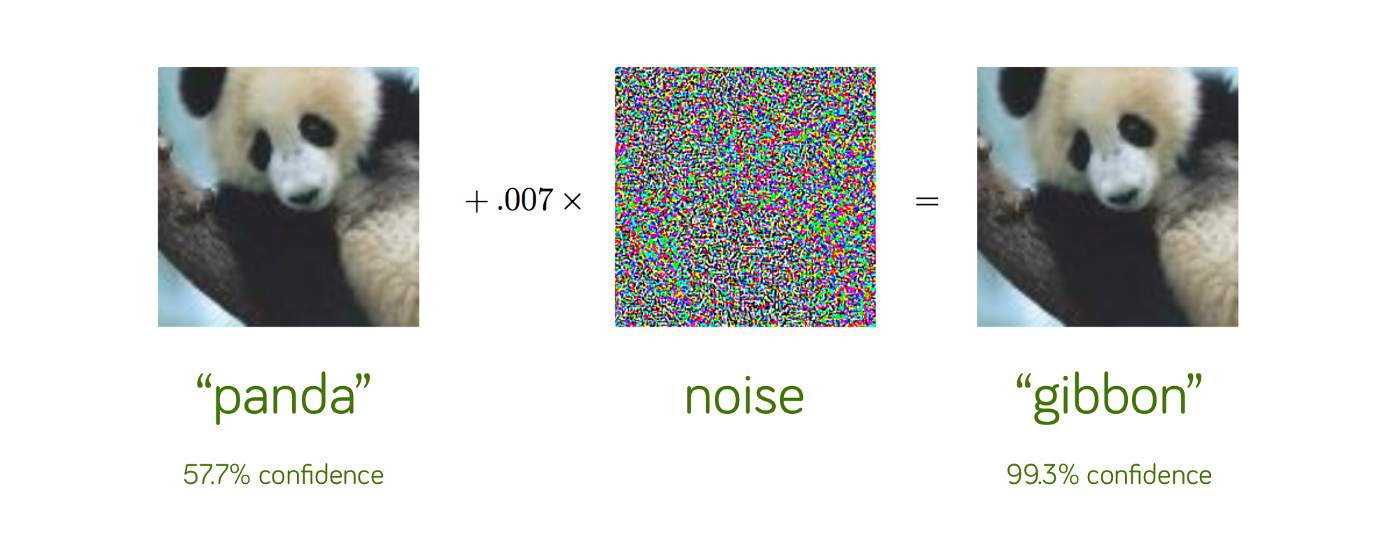
\includegraphics[scale=.12]{../images/illustrations/adversarial_attack.png}
      \end{figure}
   \end{minipage}


\end{frame}


\begin{frame}\frametitle{Python}
   \begin{minipage}{0.68\linewidth}
      \begin{itemize}
         \item Programming environment
         \item Essentials in Python language
         \begin{itemize}
            \item Data structures
            \item Control structures
            \item Functions
            \item Objects
         \end{itemize}
         \item Goog practices, coding conventions
         \item Methods to learn programming
      \end{itemize}
   \end{minipage}
   \begin{minipage}{0.28\linewidth}
      \begin{figure}[H]
         
\includegraphics[scale=.2]{../images/illustrations/github.png}
      \end{figure}
      \begin{figure}[H]
         
\includegraphics[scale=.15]{../images/illustrations/kaggle.png}
      \end{figure}
      \begin{figure}[H]
         
\includegraphics[scale=.15]{../images/illustrations/data_for_good.png}
      \end{figure}
   \end{minipage}


   \vspace{.2cm}
   \hspace{.7cm}
   \begin{minipage}{0.28\linewidth}
      \begin{figure}[H]
         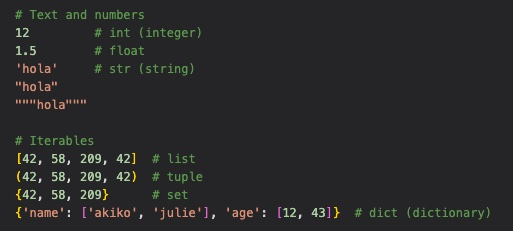
\includegraphics[scale=.3]{../images/illustrations/python_types.jpg}
      \end{figure}
   \end{minipage}
\end{frame}


\begin{frame}\frametitle{Pandas}
   \begin{figure}[H]
      \hspace{4cm}
      
\includegraphics[scale=.2]{../images/illustrations/pandas.png}
   \end{figure}
   \vspace{-1.2cm}
   \begin{itemize}
      \item Core objects
      \item Masks / Filters
      \item Basic methods (info, describe) Apply, vectorial operations
      \item Other useful methods (sort\_values, groupby, isna)
      \item Graphs (.plot, .scatter.plot, .plot.bar, .hist)
      \item merging DataFrames the right method (outer, indicator=True)
      \item Pandas profiling
   \end{itemize}

   \hspace{.5cm}
   \begin{minipage}{0.38\linewidth}
      \begin{figure}[H]
         
\includegraphics[scale=.12]{../images/illustrations/pandas_profiling.png}
      \end{figure}
   \end{minipage}
   \begin{minipage}{0.48\linewidth}
      \vspace{-.8cm}
      \begin{figure}[H]
         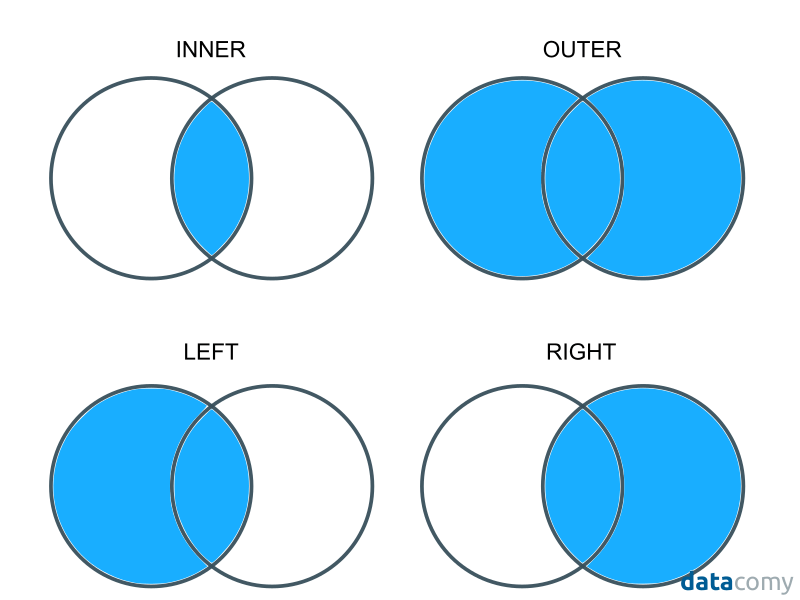
\includegraphics[scale=.13]{../images/illustrations/types_of_joins.png}
      \end{figure}
   \end{minipage}
\end{frame}


\begin{frame}\frametitle{Data Analysis}
   \begin{itemize}
      \item Measures: centrality, dispersion, IQR
      \item Pattern analysis
      \begin{itemize}
         \item Univariate
         \item Multivariate
      \end{itemize}
      \item Data type
      \begin{itemize}
         \item Qualitative, Quantitative
         \item Numbers (Times Series), text, images, music
         \item Linear, non-linear
      \end{itemize}
      \item Correlations
      \item Statistical laws and tests
   \end{itemize}

   \vspace{.2cm}
   \begin{minipage}{0.38\linewidth}
      \begin{figure}[H]
         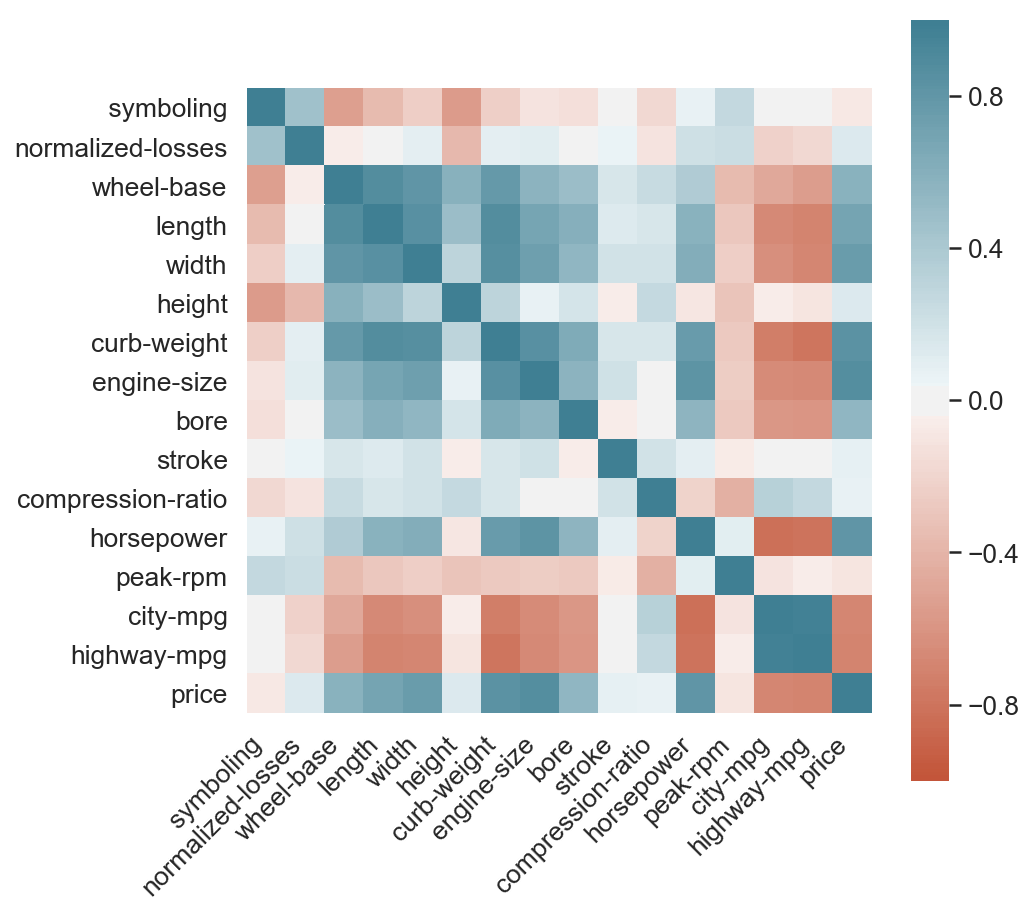
\includegraphics[scale=.07]{../images/illustrations/correlation_matrix.png}
      \end{figure}
   \end{minipage}
   \begin{minipage}{0.58\linewidth}
      \begin{figure}[H]
         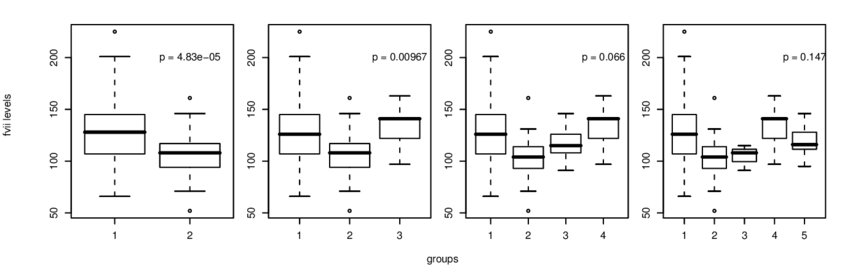
\includegraphics[scale=.22]{../images/illustrations/anova.png}
      \end{figure}
   \end{minipage}
\end{frame}


\begin{frame}\frametitle{Data Management with Pandas}
   \begin{minipage}{0.56\linewidth}
      \begin{itemize}
         \item Features selection
         \begin{itemize}
            \item Drop columns, rows\\
            (duplicates, constants, useless)
            \item Multicolinearity
         \end{itemize}
         \item NA imputation
         \begin{itemize}
            \item Missing as the information
            \item Reconstruction methods
         \end{itemize}
         \item Outliers
         \item Features transformation
         \begin{itemize}
            \item Logarithm
            \item Center and reduce
         \end{itemize}
         \item Merge, concatenate tables
         \item Feature engineering
         \begin{itemize}
            \item One-hot encode
            \item Group
            \item Filter
         \end{itemize}
      \end{itemize}
   \end{minipage}
   \begin{minipage}{0.4\linewidth}
      \begin{figure}[H]
         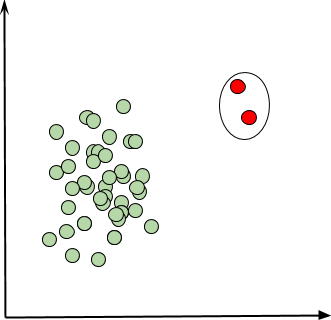
\includegraphics[scale=.21]{../images/illustrations/outliers.png}
      \end{figure}
      \begin{figure}[H]
         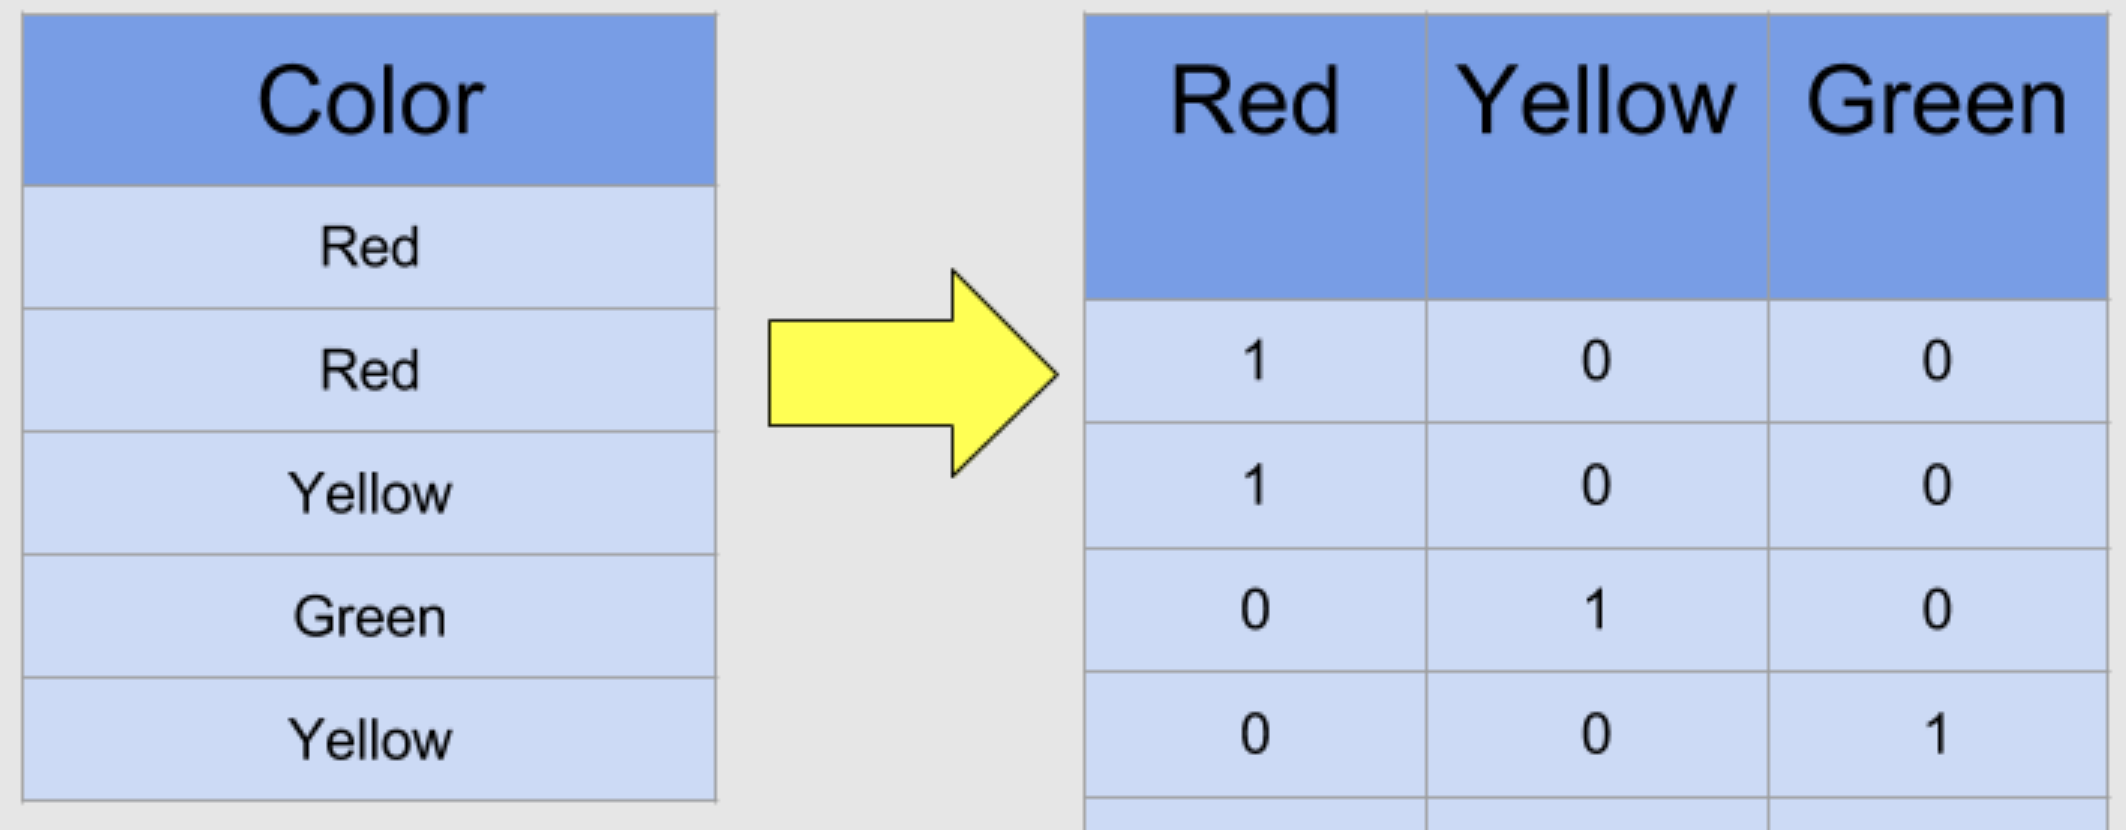
\includegraphics[scale=.11]{../images/illustrations/one_hot_encoding.png}
      \end{figure}
      \begin{figure}[H]
         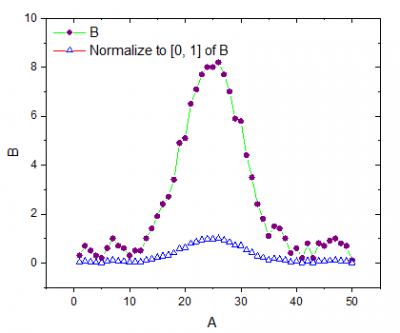
\includegraphics[scale=.23]{../images/illustrations/normalize.png}
      \end{figure}
   \end{minipage}
\end{frame}



\begin{frame}\frametitle{Data Visualization}
   \begin{minipage}{0.56\linewidth}
      \begin{itemize}
         \item Why, use cases
         \item Graph types for univariate analysis
         \begin{itemize}
            \item Histograms
            \item Line plots
            \item Lorentz Curve
         \end{itemize}
         \item Graph types for multivariate analysis
         \begin{itemize}
            \item Scatter plots
            \item Heatmaps
            \item Pairplots
         \end{itemize}
         \item Libraries
         \begin{itemize}
            \item Matplotlib
            \item Seaborn
            \item Dash
         \end{itemize}
      \end{itemize}
   \end{minipage}
   \begin{minipage}{0.4\linewidth}
      \begin{figure}[H]
         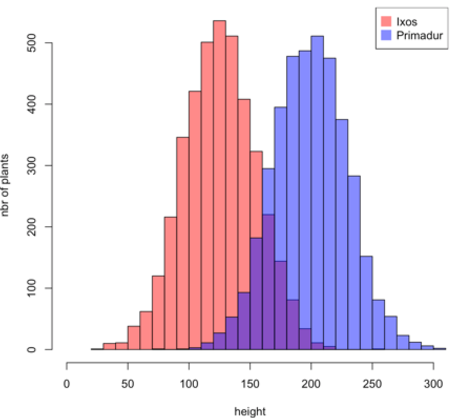
\includegraphics[scale=.21]{../src/images/illustrations/viz_histograms.png}
      \end{figure}
      \begin{figure}[H]
         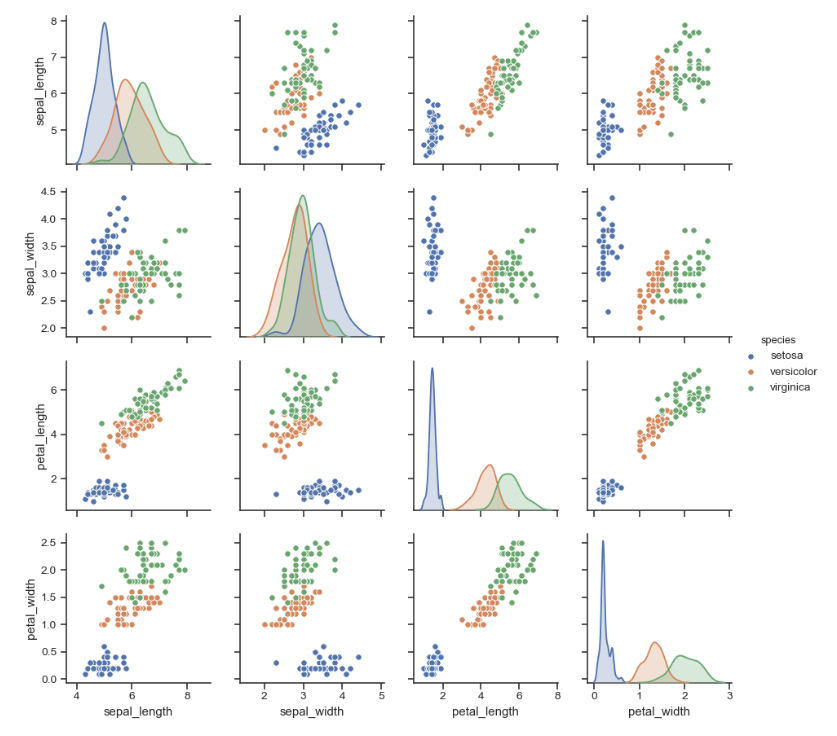
\includegraphics[scale=.12]{../images/illustrations/pairplot.png}
      \end{figure}
   \end{minipage}
\end{frame}



\begin{frame}\frametitle{Predictions}
   \begin{minipage}{0.56\linewidth}
      \begin{itemize}
         \item Correlation vs causality
         \item Use cases
         \item Regression
         \item Classification
         \item Problems types
         \begin{itemize}
            \item Supervised learning
            \item Unsupervised learning
         \end{itemize}
         \item Models
         \begin{itemize}
            \item Basic models
            \item Training
            \item Optimization
         \end{itemize}
         \item Transfer Learning
      \end{itemize}
   \end{minipage}
   \begin{minipage}{0.4\linewidth}
      \begin{figure}[H]
         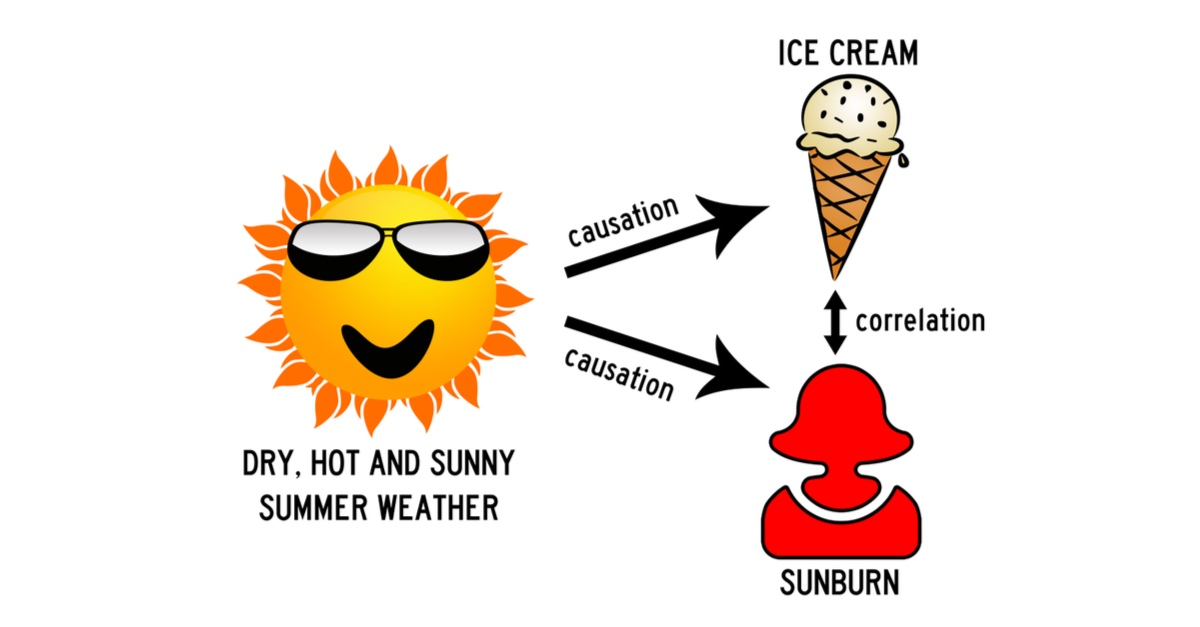
\includegraphics[scale=.11]{../images/illustrations/correlation_causality.png}
      \end{figure}
      \begin{figure}[H]
         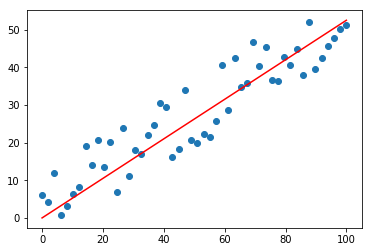
\includegraphics[scale=.22]{../images/illustrations/model_linear_regression.png}
      \end{figure}
      \begin{figure}[H]
         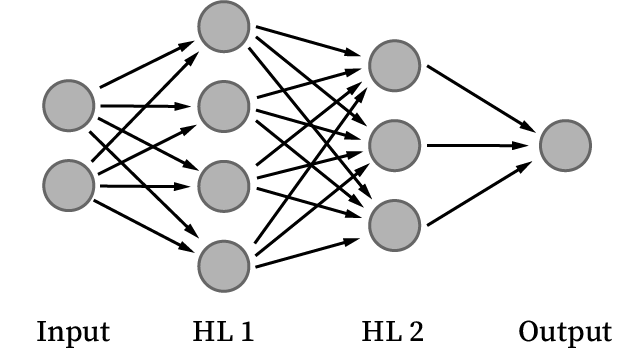
\includegraphics[scale=.17]{../images/illustrations/model_neural_network.png}
      \end{figure}
   \end{minipage}

\end{frame}




%------------------------------------------------------------------------------
\subsection{How to learn more}
%------------------------------------------------------------------------------
\begin{frame}\frametitle{How to learn more}
   \begin{itemize}
      \item Code:
      \begin{itemize}
         \item Project (personal or open source\footnote{\href{https://dataforgood.fr/}{Data for Good}})
         \item Stack Overflow
         \item \href{https://www.codingame.com/home}{Coding Game}
         \item Peers
      \end{itemize}
      \item Data Science:
      \begin{itemize}
         \item Project
         \item MOOC (Andrew Ng. Coursera - \textit{Machine Learning})
         \item Youtube channels
         \item Towards Data Science
         \item Conferences (retransmitted)
         \item Blogs of AI research Labs (GAFAM, OpenAI)
         \item Research Papers
         \item Books
      \end{itemize}
      \item Be confident: the harder it is, the stronger your comprehension\footnote{"Make It Stick: The Science of Successful Learning" - Peter C. Brown}
   \end{itemize}
\end{frame}


%------------------------------------------------------------------------------
\subsection{Job Market}
%------------------------------------------------------------------------------
\begin{frame}\frametitle{Job Market}
   \begin{itemize}
      \item Your current job might need your skills (automating, analysis, clustering, prediction)
      \item Data Analyst
      \item Data Scientist
      \item Data Engineer
      \item Machine Learning Engineer
      \item Project Manager
      \item Researcher
      \item Developer
      \item Sales
      \item Better communication with developers
   \end{itemize}
\end{frame}

%------------------------------------------------------------------------------
\subsection{Questions}
%------------------------------------------------------------------------------
\begin{frame}\frametitle{Questions}
   \begin{itemize}
      \item What are your questions?
   \end{itemize}
\end{frame}


% \begin{frame}\frametitle{Useful references}
%    \begin{itemize}
%       \item \href{https://github.com/dformoso/machine-learning-mindmap/blob/master/Machine%20Learning.pdf}{Data Science mind maps}
%       \item \href{https://github.com/josephmisiti/awesome-machine-learning}{List of tools and ressources for machine learning}
%       \item \href{https://paperswithcode.com/sota}{papers with code}
%    \end{itemize}
% \end{frame}


\end{document}
